\section{Inngangur}
Við ákváðum að búa til eftirlits róbot. Í grunninn á vélmennið að fara hring í kringum tiltekið
svæði og taka upp allt sem verður í vegi þess. Ástæðan fyrir því að við völdum þetta verkefni
er því það er mjög sveigjanlegt og ekki flókið að fá grunn virknina til að virka. Síðan þegar
það er komið er hægt að bæta við allskonar eiginleikum sem bæta virkni vélmennisins. Þær 
hugmyndir sem við höfum fengið og munum bæta við eftir því hversu mikin tíma við höfum eru t.d.
leyfa manneskju að stýra vélmenninu með appi, láta myndavélina geta hreyfst í margar áttir,
Gera vélmenninu kleift að keyra sjálfur án þess að klessa á neitt og komast aftur á rétta braut
ef það þurfti að sveigja hjá einhverju, láta vélmennið þekkja sitt svæði og senda út viðvörun
ef hann skynjar einhverja breytingu. Mismunandi og misflóknar aðferðir við að leysa margt að
þessu sem gerir þetta að skemmtilegu og krefjandi verkefni án þess þó að enda með ekki neitt
í höndunum. \cite{cite1}
\begin{figure}[h]
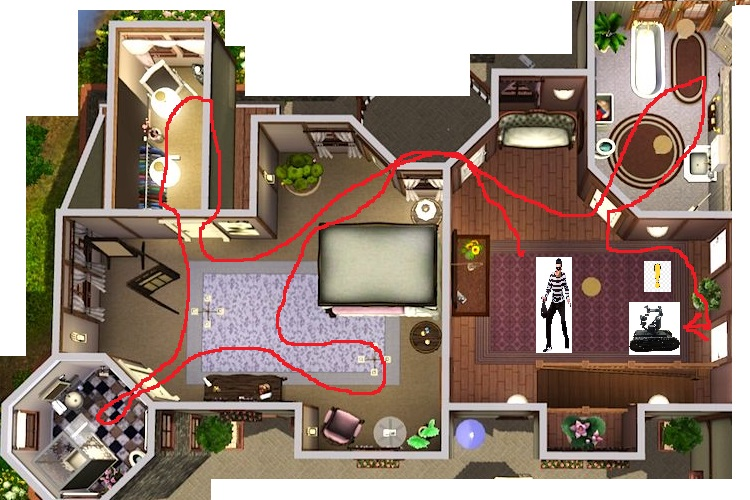
\includegraphics[scale=.4]{img/husmynd}
\end{figure}